% !TeX root = ../paper.tex
\begin{figure}[!htbp]
\centering
\setlength{\parskip}{0pt}
\setlength{\abovecaptionskip}{\baselineskip}
\setlength{\belowcaptionskip}{0pt}
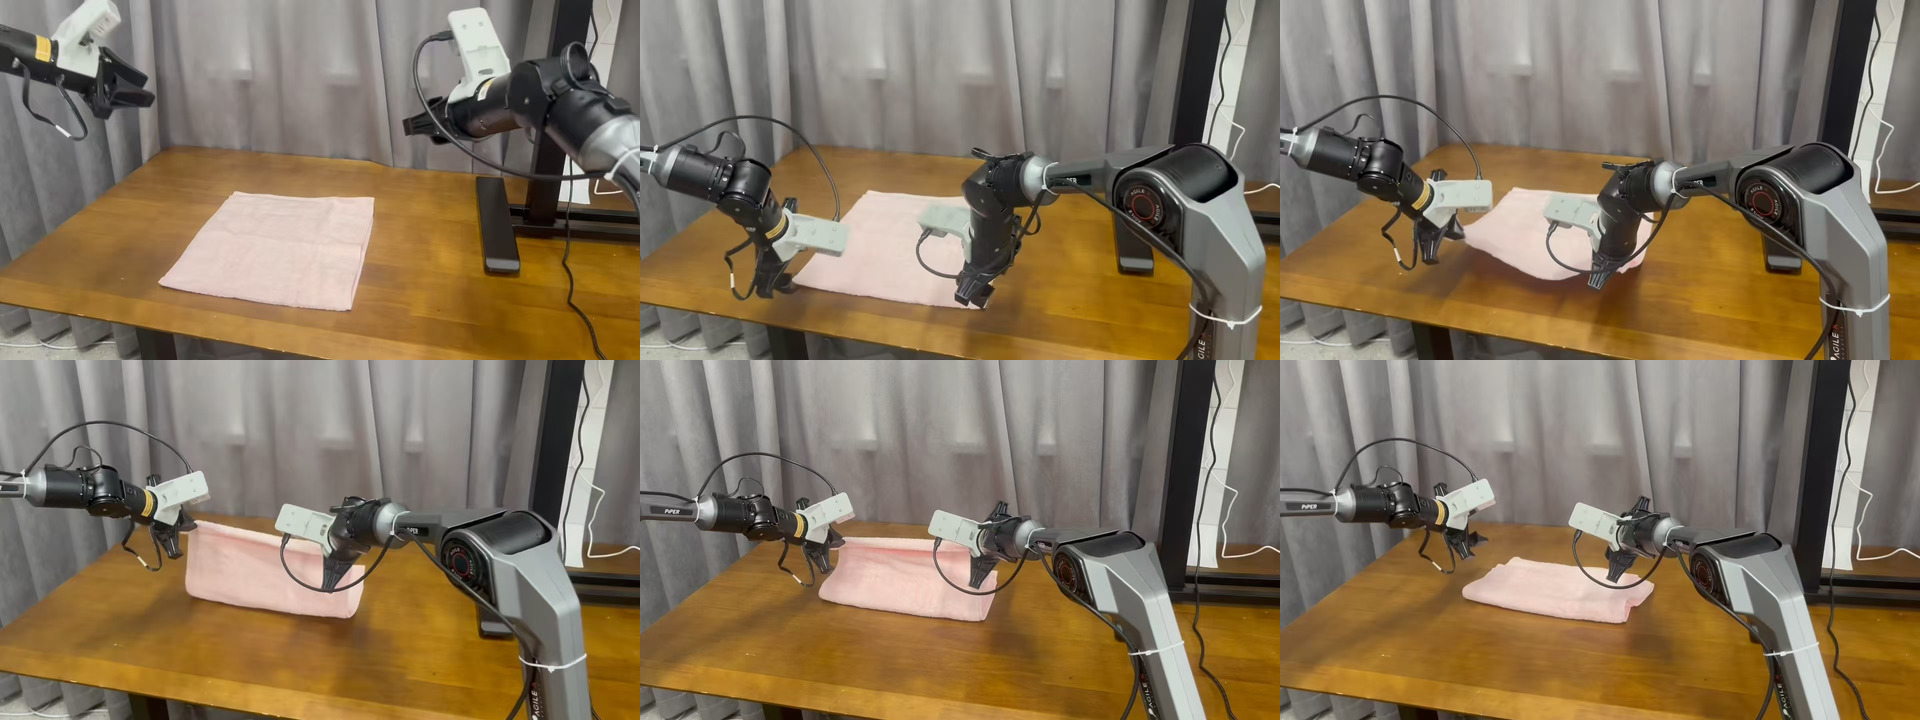
\includegraphics[width=.95\linewidth]{figures/piper_trajectories/towel_contact_sheet.jpg}\par\nointerlineskip
\caption{Piper Semantic task execution. Task instruction: ``Fold the towel from bottom to top.''}
\label{fig:piper-semantic-trajectory}
\par\vspace{\baselineskip}\nointerlineskip
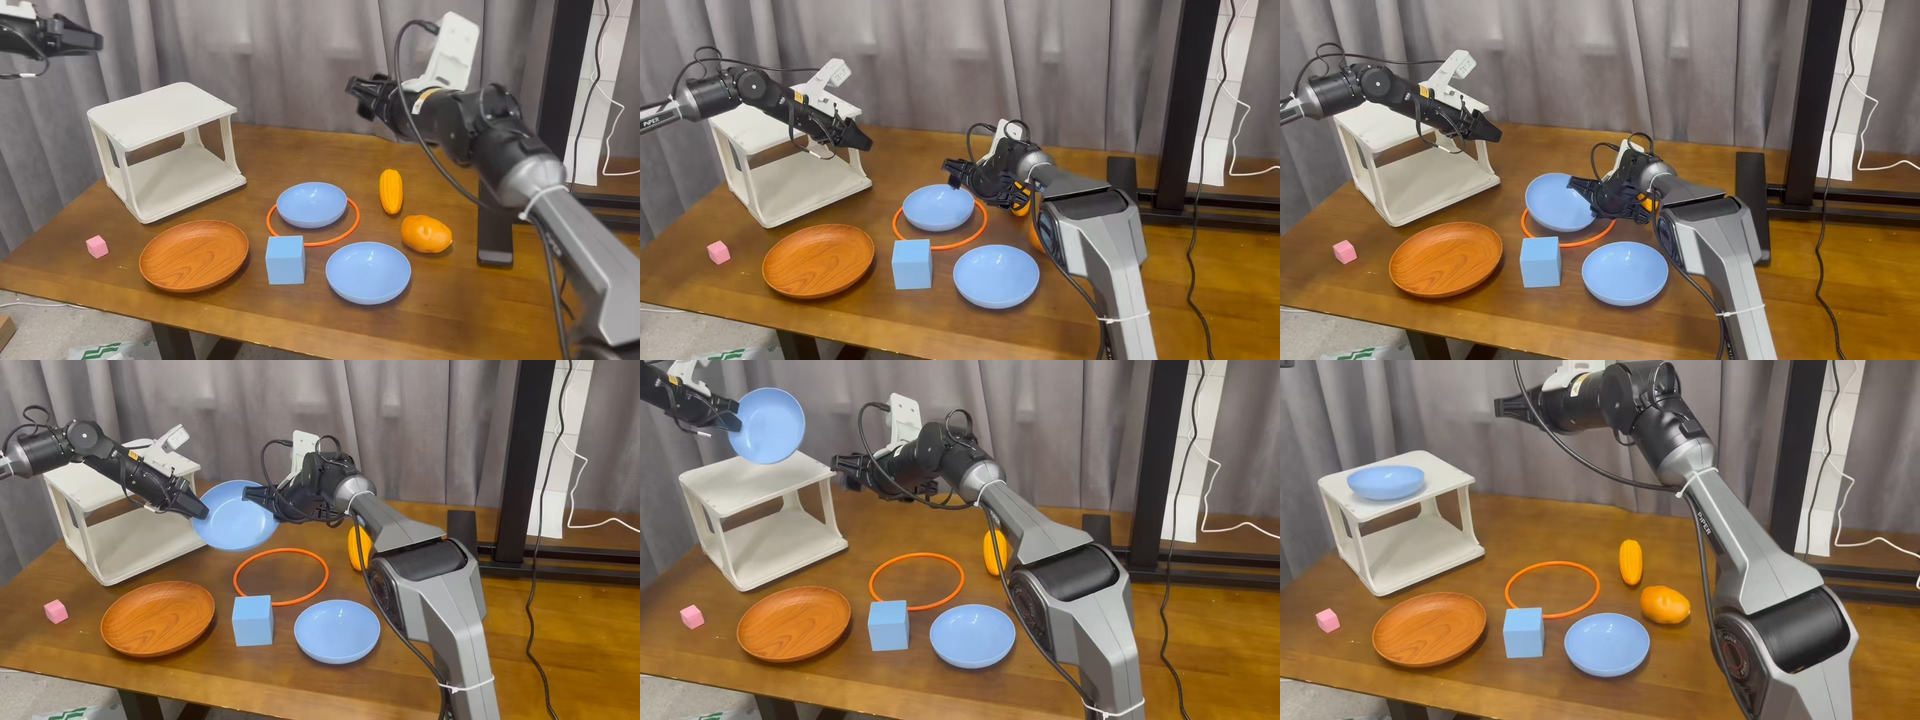
\includegraphics[width=.95\linewidth]{figures/piper_trajectories/spatial_contact_sheet.jpg}\par\nointerlineskip
\caption{Piper Visual Prompt task execution. Task instruction: ``Place the bowl marked by the red circle on the shelf.''}
\label{fig:piper-vis-trajectory}
\par\vspace{\baselineskip}\nointerlineskip
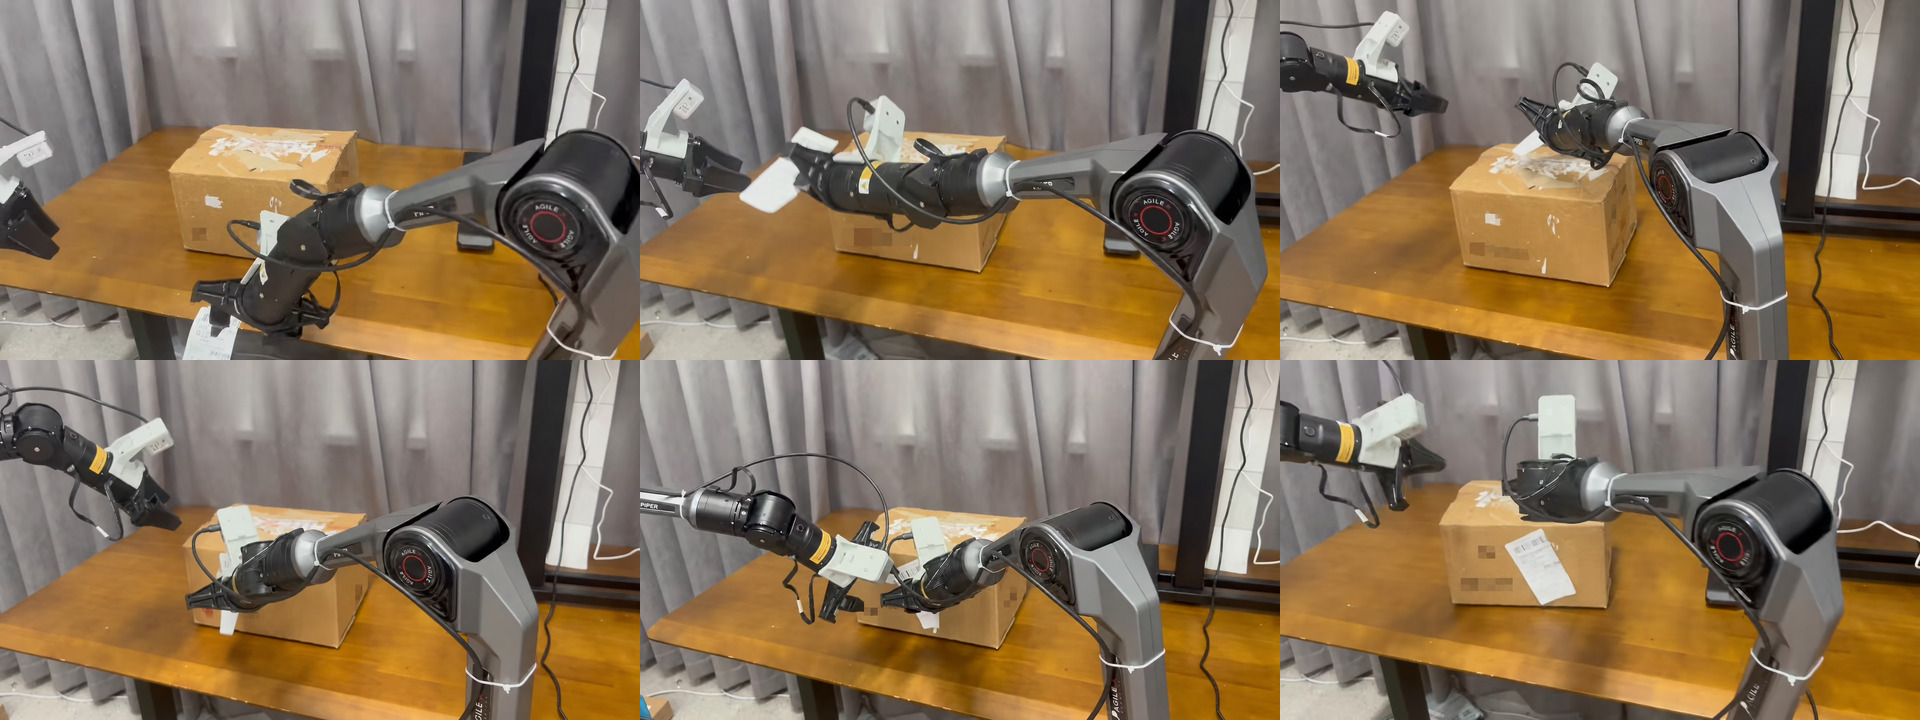
\includegraphics[width=.95\linewidth]{figures/piper_trajectories/control_contact_sheet.jpg}\par\nointerlineskip
\caption{Piper Control task execution. The initial instruction, ``Attach the sticker to the top of the box,'' is replaced during execution by ``Attach the sticker to the front of the box.''}
\label{fig:piper-control-trajectory}
\end{figure}
